\documentclass[12pt, titlepage]{article}

\usepackage{fullpage}
\usepackage[round]{natbib}
\usepackage{multirow}
\usepackage{booktabs}
\usepackage{tabularx}
\usepackage{graphicx}
\usepackage{float}
\usepackage{hyperref}
\hypersetup{
    colorlinks,
    citecolor=blue,
    filecolor=black,
    linkcolor=red,
    urlcolor=blue
}


\newcounter{acnum}
\newcommand{\actheacnum}{AC\theacnum}
\newcommand{\acref}[1]{AC\ref{#1}}

\newcounter{ucnum}
\newcommand{\uctheucnum}{UC\theucnum}
\newcommand{\uref}[1]{UC\ref{#1}}

\newcounter{mnum}
\newcommand{\mthemnum}{M\themnum}
\newcommand{\mref}[1]{M\ref{#1}}

\begin{document}

\title{Module Guide for Retinal Vessel Segmentation System (RVSS)}
 
\author{Xinyu Ma}
\date{March 18, 2024}

\maketitle

\pagenumbering{roman}

\section{Revision History}

\begin{tabularx}{\textwidth}{p{3cm}p{2cm}X}
\toprule {\bf Date} & {\bf Version} & {\bf Notes}\\
\midrule
03/13/2024 & 1.0 & Initial Release  \\

\bottomrule
\end{tabularx}

\newpage

\section{Reference Material}

This section records information for easy reference.

\subsection{Abbreviations and Acronyms}

\renewcommand{\arraystretch}{1.2}
\begin{tabular}{l l} 
  \toprule		
  \textbf{symbol} & \textbf{description}\\
  \midrule 
  AC & Anticipated Change\\
  CNN & Convolution Neural Network\\
  DAG & Directed Acyclic Graph \\
  M & Module \\
  MG & Module Guide \\
  OS & Operating System \\
  R & Requirement\\
  RVSS & Retinal Vessel Segmentation System \\ 
  SRS & Software Requirements Specification\\
  UC & Unlikely Change \\
  \bottomrule
\end{tabular}\\
For complete symbols, abbreviations and acronyms used within the system, please refer the section 1.3 in \href{https://github.com/lele0007/Blood-vessel-segmentation/blob/main/docs/SRS/SRS.pdf}{SRS} document.
\newpage

\tableofcontents

\listoftables

\listoffigures

\newpage

\pagenumbering{arabic}

\section{Introduction}

Decomposing a system into modules is a commonly accepted approach to developing software. A module is a work assignment for a programmer or programming team~\citep{parnas1985modular}. We advocate a decomposition based on the principle of information hiding~\citep{parnas1972criteria}. This principle supports design for change, because the ``secrets'' that each module hides represent likely future changes. Design for change is valuable in SC, where modifications are frequent, especially during initial development as the solution space is explored.  

Our design follows the rules layed out by \citet{parnas1985modular}, as follows:
\begin{itemize}
\item System details that are likely to change independently should be the secrets of separate modules.
\item Each data structure is implemented in only one module.
\item Any other program that requires information stored in a module's data structures must obtain it by calling access programs belonging to that module.
\end{itemize}

After completing the first stage of the design, the Software Requirements Specification (SRS), the Module Guide (MG) is developed~\citep{parnas1985modular}. The MG specifies the modular structure of the system and is intended to allow both
designers and maintainers to easily identify the parts of the software. The potential readers of this document are as follows:

\begin{itemize}
\item New project members: This document can be a guide for a new project member to easily understand the overall structure and quickly find the relevant modules they are searching for.
\item Maintainers: The hierarchical structure of the module guide improves the maintainers' understanding when they need to make changes to the system. It is important for a maintainer to update the relevant sections of the document after changes have been made.
\item Designers: Once the module guide has been written, it can be used to check for consistency, feasibility, and flexibility. Designers can verify the system in various ways, such as consistency among modules, feasibility of the
  decomposition, and flexibility of the design.
\end{itemize}

The rest of the document is organized as follows. Section \ref{SecChange} lists the anticipated and unlikely changes of the software requirements. Section \ref{SecMH} summarizes the module decomposition that was constructed according to the likely changes. Section \ref{SecConnection} specifies the connections between the software requirements and the
modules. Section \ref{SecMD} gives a detailed description of the modules. Section \ref{SecTM} includes two traceability matrices. One checks the completeness of the design against the requirements provided in the SRS. The other shows the relation between anticipated changes and the modules. Section \ref{SecUse} describes the use relation between modules.

\section{Anticipated and Unlikely Changes} \label{SecChange}

This section lists possible changes to the system. According to the likeliness of the change, the possible changes are classified into two categories. Anticipated changes are listed in Section \ref{SecAchange}, and unlikely changes are listed in Section \ref{SecUchange}.

\subsection{Anticipated Changes} \label{SecAchange}

Anticipated changes are the source of the information that is to be hidden inside the modules. Ideally, changing one of the anticipated changes will only require changing the one module that hides the associated decision. The approach
adapted here is called design for change. This "design for change" approach ensures that when updates or modifications are needed, they can be managed within the scope of a single module, minimizing the impact on the overall system. Below are the anticipated changes that have been considered in the development of RVSS, along with the modules that would encapsulate these change.

\begin{description}
\item[\refstepcounter{acnum} \actheacnum \label{1_ac}:] The specific hardware specifications or configurations on which the software is running.
\begin{itemize}
    \item Encapsulated in: Hardware-Hiding Module
    \item Rationale: Adds portability to the software since not everyone has the same hardware to run it on and allows for hardware upgrades or changes without affecting the rest of the system..
\end{itemize}
\item[\refstepcounter{acnum} \actheacnum \label{2_ac}:] The image preprocessing algorithms.New or improved algorithms for image normalization, denoising, and contrast enhancement may become available.
\begin{itemize}
    \item Encapsulated in: Image Preprocessing Module
    \item Rationale: By isolating image preprocessing algorithms within this module, updates algorithms can be made without affecting the segmentation process or other system components.
\end{itemize}

\item[\refstepcounter{acnum} \actheacnum \label{3_ac}:] The image segmentation algorithms. Advances in image segmentation algorithms, including machine learning models, could offer enhanced accuracy or efficiency.
\begin{itemize}
    \item Encapsulated in: Image Segmentation Module
    \item Rationale: Encapsulating segmentation algorithms within its module allows for straightforward integration of new algorithms or updates to existing ones, facilitating continuous improvement in segmentation performance.
\end{itemize}
\item[\refstepcounter{acnum} \actheacnum \label{4_ac}:] Reporting Formats and Contents
\begin{itemize}
    \item Encapsulated in: Report Generation Module
    \item Rationale: Encapsulating report generation within its module allows for modifications to report formats, contents, or additional data visualization techniques without affecting other system components.
\end{itemize}

\item[\refstepcounter{acnum} \actheacnum \label{5_ac}:] Image data storage methods.
\begin{itemize}
    \item Encapsulated in: Image Management Module
    \item Rationale: Encapsulating data storage allows for changes in underlying storage solutions or adaptation to new data management practices without impacting other system functionalities.
\end{itemize}

\item[\refstepcounter{acnum} \actheacnum \label{6_ac}:] Updates the user interface design principles or the introduction of new user interaction models.
\begin{itemize}
    \item Encapsulated in: User Interface Module
    \item Rationale: User Interface trends change over time and encapsulating user interface within a dedicated module allows for updates and redesigns to be carried out with minimal disruption.
\end{itemize}
\end{description}

\subsection{Unlikely Changes} \label{SecUchange}

The module design should be as general as possible. However, a general system is more complex. Sometimes this complexity is not necessary. Fixing some design decisions at the system architecture stage can simplify the software design. If these decision should later need to be changed, then many parts of the design will potentially need to be modified. Hence, it is not intended that these decisions will be changed.

\begin{description}
\item[\refstepcounter{ucnum} \uctheucnum \label{ucIO_1}:] Fundamental image input formats: The decision to support standard fundus image formats (e.g., JPEG, PNG) is unlikely to change. Expanding to different or proprietary image formats would necessitate considerable adjustments in preprocessing algorithms and data management methods.
\item[\refstepcounter{ucnum} \uctheucnum \label{ucInput_2}:] Primary programming language: The choice of programming language (i.e., Python) for the RVSS development has implications for performance optimization, library availability and compatibility. A change in the primary programming language is considered unlikely due to the extensive effort required to rewrite and retest the system.
\item[\refstepcounter{ucnum} \uctheucnum \label{ucOutput_3}:] The core system architecture: The modular architecture of RVSS, including the division of functionalities into specific modules, is a foundational design choice unlikely to undergo radical changes. 
\item[\refstepcounter{ucnum} \uctheucnum \label{ucEnergy_4}:] The goal of RVSS is to generate vessel segmentation maps of fundus images, which is unlikely to change.

\end{description}

\section{Module Hierarchy} \label{SecMH}

This section provides an overview of the module design. Modules are summarized
in a hierarchy decomposed by secrets in Table \ref{TblMH}. The modules listed
below, which are leaves in the hierarchy tree, are the modules that will
actually be implemented.

\begin{description}
\item [\refstepcounter{mnum} \mthemnum \label{1_mHH}:] Hardware-Hiding Module
\item [\refstepcounter{mnum} \mthemnum \label{2_mHH}:] Input Upload and Validate Module
\item [\refstepcounter{mnum} \mthemnum \label{3_mHH}:] Image Management Module
\item [\refstepcounter{mnum} \mthemnum \label{4_mHH}:] Image Preprocessing Module
\item [\refstepcounter{mnum} \mthemnum \label{5_mHH}:] Image Segmentation Module
\item [\refstepcounter{mnum} \mthemnum \label{6_mHH}:] Output Format Module
\item [\refstepcounter{mnum} \mthemnum \label{7_mHH}:] Report Generation Module
\item [\refstepcounter{mnum} \mthemnum \label{8_mHH}:] User Interface Module
\item [\refstepcounter{mnum} \mthemnum \label{9_mHH}:] Main Function Module
\item [\refstepcounter{mnum} \mthemnum \label{10_mHH}:] Algorithm Optimization Module
\item [\refstepcounter{mnum} \mthemnum \label{11_mHH}:] Plotting Result Module
\item [\refstepcounter{mnum} \mthemnum \label{12_mHH}:] Logging Module
\item [\refstepcounter{mnum} \mthemnum \label{13_mHH}:] Image patching Module 
\item [\refstepcounter{mnum} \mthemnum \label{14_mHH}:] Image Dataset Reader Module 
\item [\refstepcounter{mnum} \mthemnum \label{15_mHH}:] Network Model Reader Module 

\end{description}


\begin{table}[h!]
\centering
\begin{tabular}{p{0.3\textwidth} p{0.6\textwidth}}
\toprule
\textbf{Level 1} & \textbf{Level 2}\\
\midrule
{Hardware-Hiding Module} & ~ \\
\midrule

\multirow{7}{0.3\textwidth}{Behaviour-Hiding Module} 
& Input Upload and Validate Module\\ 
& Image Management Module\\
& Image Preprocessing Module\\
& Image Segmentation Module\\
& Output Format Module\\
& Report Generation Module\\
& User Interface Module\\
& Main Function Module\\
\midrule

\multirow{3}{0.3\textwidth}{Software Decision Module} 
& Algorithm Optimization Module\\
& Plotting Result Module\\
& Logging Module\\
& Image patching Module\\
& Image Dataset Reader Module\\
& Network Model Reader Module\\
\bottomrule

\end{tabular}
\caption{Module Hierarchy}
\label{TblMH}
\end{table}

\section{Connection Between Requirements and Design} \label{SecConnection}

The design of the system is intended to satisfy the requirements developed in the SRS. In this stage, the system is decomposed into modules. The connection between requirements and modules is listed in Table~\ref{TblRT}.

\section{Module Decomposition} \label{SecMD}

Modules are decomposed according to the principle of ``information hiding'' proposed by \citet{parnas1985modular}. The \emph{Secrets} field in a module decomposition is a brief statement of the design decision hidden by the
module. The \emph{Services} field specifies \emph{what} the module will do without documenting \emph{how} to do it. For each module, a suggestion for the implementing software is given under the \emph{Implemented By} title. If the entry is \emph{OS}, this means that the module is provided by the operating system or by standard programming language libraries.  \emph{RVSS} means the module will be implemented by the RVSS software.

Only the leaf modules in the hierarchy have to be implemented. If a dash (\emph{--}) is shown, this means that the module is not a leaf and will not have to be implemented.

\subsection{Hardware Hiding Modules (\mref{1_mHH})}

\begin{description}
\item[Secrets:]The data structure, algorithm and underlying hardware used to implement the virtual hardware.
\item[Services:]Serves as a virtual hardware used by the rest of the system. This module provides the interface between the hardware and the software. So, the system can use it to display outputs or to accept inputs.
\item[Implemented By:] OS
\end{description}


\subsection{Behaviour-Hiding Module}

\begin{description}
\item[Secrets:]The contents of the required behaviours.
\item[Services:]Includes programs that provide externally visible behaviour of the system as specified in the software requirements specification (\href{https://github.com/lele0007/Blood-vessel-segmentation/blob/main/docs/SRS/SRS.pdf}{SRS}) documents. This module serves as a communication layer between the hardware-hiding module and the software decision module. The programs in this module will need to change if there are changes in the SRS.
\item[Implemented By:] \emph{--}
\end{description}

\subsubsection{Input Upload and Validate Module (\mref{2_mHH})}
\begin{description}
\item[Secrets:] The processes and validations involved in uploading images within the system.
\item[Services:] Provides functionalities for users to upload fundus images and ensures that uploaded images meet specified format and quality criteria.
\item[Implemented By:] RVSS
\item[Type of Module:] Abstract Object
\end{description}


\subsubsection{Image Management Module (\mref{3_mHH})}
\begin{description}
\item[Secrets:] The processes and validations involved in storing and managing fundus images within the system.
\item[Services:] Provides functionalities for users to manage stored images, and retrieve them for processing.
\item[Implemented By:] RVSS
\item[Type of Module:] Record
\end{description}



\subsubsection{Image Preprocessing Module (\mref{4_mHH})}
\begin{description}
\item[Secrets:] The algorithms for image normalization, denoising, and contrast enhancement.
\item[Services:] Prepares images for segmentation by improving their quality and standardizing their format.
\item[Implemented By:] RVSS
\item[Type of Module:] Library
\end{description}

\subsubsection{Image Segmentation Module (\mref{5_mHH})}

\begin{description}
\item[Secrets:] The specific machine learning algorithms and techniques used to identify and delineate retinal vessels from the preprocessed fundus images.
\item[Services:] Segments retinal vessels from the preprocessed fundus images.
\item[Implemented By:] RVSS
\item[Type of Module:] Library
\end{description}

\subsubsection{Output Format Module (\mref{6_mHH})}
\begin{description}
\item[Secrets:] The format and structure of the output.
\item[Services:] Outputs the results of the segmentation, including the input image and the corresponding image with only blood vessels (white pixels) and background (black pixels). 
\item[Implemented By:] RVSS
\item[Type of Module:] Abstract Object
\end{description}

\subsubsection{Report Generation Module (\mref{7_mHH})}
\begin{description}
\item[Secrets:] The format, layout, and content inclusion criteria for generating reports.
\item[Services:] Compiles the input image, the segmentation results and analyses into structured reports.
\item[Implemented By:] RVSS
\item[Type of Module:] Abstract Object
\end{description}

\subsubsection{User Interface Module (\mref{8_mHH})}
\begin{description}
\item[Secrets:] The design and workflow of the graphical user interface.
\item[Services:] Provides an interface for users to interact with the system, from uploading fundus images to viewing reports.
\item[Implemented By:] RVSS
\item[Type of Module:] Abstract Object
\end{description}

\subsubsection{Main Function Module (\mref{9_mHH})}
\begin{description}
\item[Secrets:] The algorithm for coordinating the running of the program.
\item[Services:] Provides the main function of the system which uses the services that are provided by other modules to upload fundus images, preprocess the original fundus images, segment retinal vessels from the preprocessed fundus images, and generate output images and report. 
\item[Implemented By:] RVSS
\item[Type of Module:] Abstract Data Type
\end{description}

\subsection{Software Decision Module}

\begin{description}
\item[Secrets:] The design decision based on mathematical theorems, physical facts, or programming considerations. The secrets of this module are \emph{not} described in the SRS.
\item[Services:] Includes data structure and algorithms used in the system that
  do not provide direct interaction with the user. 
\item[Implemented By:] --
\end{description}

\subsubsection{Algorithm Optimization Module(\mref{10_mHH})}
\begin{description}
\item[Secrets:]Specific optimization techniques and algorithms used to enhance the performance of image processing and segmentation tasks.
\item[Services:]Provides optimized processing for image preprocessing and segmentation, reducing computation time and resource usage.
\item[Implemented By:] PyTorch
\item[Type of Module:] Library
\end{description}

\subsubsection{Plotting Result Module (\mref{11_mHH})}
\begin{description}
\item[Secrets:] Plots the data and algorithms graphically.
\item[Services:] Provides function that can accept the output of the segmentation algorithm and plot the results using in the output format module and the report generation module. 
\item[Implemented By:] torchvision,tensorboard
\item[Type of Module:] Library
\end{description}

\subsubsection{Logging Module (\mref{12_mHH})}
\begin{description}
\item[Secrets:] The specific algorithms and configurations used for log message formatting, storage, categorization by severity levels, and handling of log data persistence and retrieval without impacting system performance or resource utilization.
\item[Services:] Delivers essential system-wide services that enhance the maintainability and operability of the system, including logging services for debugging and audit trails.
\item[Implemented By:] RVSS or OS (for standard functionalities provided by the operating system or python libraries)
\item[Type of Module:] Library
\end{description}

\subsubsection{Image patching Module (\mref{13_mHH})}
\begin{description}
\item[Secrets:] The methods to divide the image into multiple small patches. 
\item[Services:] Provides data for the process of neural network learning and training. 
\item[Implemented By:] PyTorch 
\item[Type of Module:] Library
\end{description}

\subsubsection{Image Dataset Reader Module(\mref{14_mHH})}
\begin{description}
\item[Secrets:]The algorithm to read fundus training dataset and test dataset. 
\item[Services:] Provides images that can be used for model training and testing. 
\item[Implemented By:] PyTorch
\item[Type of Module:] Library
\end{description}

\subsubsection{Network Model Reader Module(\mref{15_mHH})}
\begin{description}
\item[Secrets:]Load the model parameters of the pre-trained neural network.
\item[Services:] Provide model parameters for the testing phase
\item[Implemented By:] PyTorch
\item[Type of Module:] Library
\end{description}





\section{Traceability Matrix} \label{SecTM}

This section shows two traceability matrices: between the modules and the requirements and between the modules and the anticipated changes.

% the table should use mref, the requirements should be named, use something
% like fref
\begin{table}[H]
\centering
\begin{tabular}{p{0.2\textwidth} p{0.6\textwidth}}
\toprule
\textbf{Req.} & \textbf{Modules}\\
\midrule
R1 & \mref{2_mHH}, \mref{3_mHH}, \mref{8_mHH}, \mref{9_mHH}\\
R3 & \mref{3_mHH}, \mref{4_mHH}, \mref{9_mHH}, \mref{12_mHH}, \mref{14_mHH}\\
R4 & \mref{1_mHH}, \mref{5_mHH}, \mref{9_mHH}, \mref{10_mHH}, \mref{12_mHH}, \mref{13_mHH}, \mref{14_mHH}, \mref{15_mHH}\\
R5 & \mref{6_mHH}, \mref{7_mHH},  \mref{8_mHH}, \mref{9_mHH},\mref{11_mHH}, \mref{12_mHH}\\
\bottomrule
\end{tabular}
\caption{Trace Between Requirements and Modules}
\label{TblRT}
\end{table}

\begin{table}[H]
\centering
\begin{tabular}{p{0.2\textwidth} p{0.6\textwidth}}
\toprule
\textbf{AC} & \textbf{Modules}\\
\midrule
\acref{1_ac} & \mref{1_mHH}\\
\acref{2_ac} & \mref{4_mHH}\\
\acref{3_ac} & \mref{5_mHH}\\
\acref{4_ac} & \mref{7_mHH}\\
\acref{5_ac} & \mref{3_mHH}\\
\acref{6_ac} & \mref{8_mHH}\\

\bottomrule
\end{tabular}
\caption{Trace Between Anticipated Changes and Modules}
\label{TblACT}
\end{table}

\section{Use Hierarchy Between Modules} \label{SecUse}

In this section, the uses hierarchy between modules is provided. Parnas \cite{parnas1979designing} said of two programs A and B that A {\em uses} B if correct execution of B may be necessary for A to complete the task described in its specification. That is, A {\em uses} B if there exist situations in which the correct functioning of A depends upon the availability of a correct implementation of B.  Figure \ref{Fig1} illustrates the use relation between the modules. It can be seen that the graph is a directed acyclic graph (DAG). Each level of the hierarchy offers a testable and usable subset of the system, and modules in the higher level of the hierarchy are essentially simpler because they use modules from the lower levels.

Assume that the model is mainly used for application rather than development (training a own model to use), so before using the model, we will pre-train a model, and then call the main function for user use.

\begin{figure}[H]
\centering
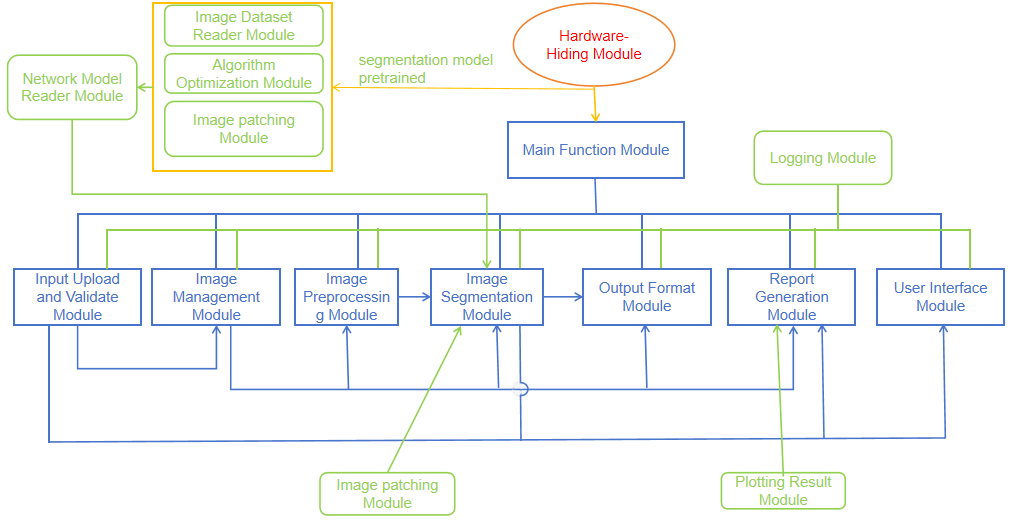
\includegraphics[width=0.9\textwidth]{1.png}
\caption{Use Hierarchy Among Modules}
\label{Fig1}
\end{figure}

%\section*{References}
\newpage
\bibliographystyle {plain}
\bibliography {ref}

\newpage{}

\end{document}